% Created by tikzDevice version 0.10.1 on 2016-09-01 16:11:35
% !TEX encoding = UTF-8 Unicode
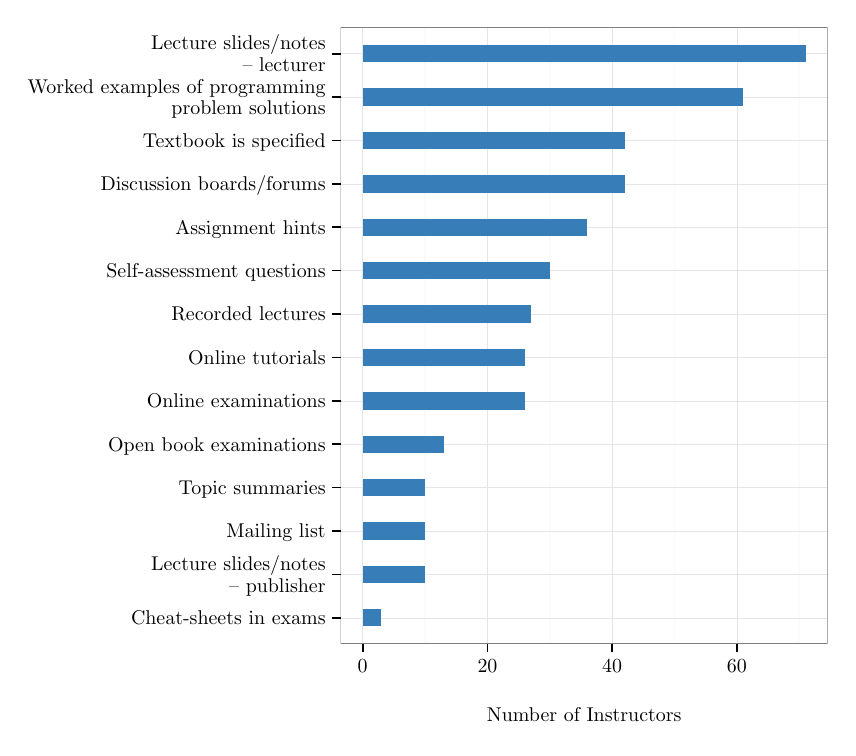
\begin{tikzpicture}[x=1pt,y=1pt]
\definecolor{fillColor}{RGB}{255,255,255}
\path[use as bounding box,fill=fillColor,fill opacity=0.00] (0,0) rectangle (289.08,252.94);
\begin{scope}
\path[clip] (  0.00,  0.00) rectangle (289.08,252.94);
\definecolor{drawColor}{RGB}{255,255,255}
\definecolor{fillColor}{RGB}{255,255,255}

\path[draw=drawColor,line width= 0.6pt,line join=round,line cap=round,fill=fillColor] (  0.00,  0.00) rectangle (289.08,252.95);
\end{scope}
\begin{scope}
\path[clip] (113.07, 30.29) rectangle (289.08,252.94);
\definecolor{fillColor}{RGB}{255,255,255}

\path[fill=fillColor] (113.07, 30.29) rectangle (289.08,252.94);
\definecolor{drawColor}{gray}{0.98}

\path[draw=drawColor,line width= 0.6pt,line join=round] (143.61, 30.29) --
	(143.61,252.94);

\path[draw=drawColor,line width= 0.6pt,line join=round] (188.68, 30.29) --
	(188.68,252.94);

\path[draw=drawColor,line width= 0.6pt,line join=round] (233.75, 30.29) --
	(233.75,252.94);

\path[draw=drawColor,line width= 0.6pt,line join=round] (278.83, 30.29) --
	(278.83,252.94);
\definecolor{drawColor}{gray}{0.90}

\path[draw=drawColor,line width= 0.2pt,line join=round] (113.07, 39.70) --
	(289.08, 39.70);

\path[draw=drawColor,line width= 0.2pt,line join=round] (113.07, 55.38) --
	(289.08, 55.38);

\path[draw=drawColor,line width= 0.2pt,line join=round] (113.07, 71.06) --
	(289.08, 71.06);

\path[draw=drawColor,line width= 0.2pt,line join=round] (113.07, 86.74) --
	(289.08, 86.74);

\path[draw=drawColor,line width= 0.2pt,line join=round] (113.07,102.42) --
	(289.08,102.42);

\path[draw=drawColor,line width= 0.2pt,line join=round] (113.07,118.10) --
	(289.08,118.10);

\path[draw=drawColor,line width= 0.2pt,line join=round] (113.07,133.78) --
	(289.08,133.78);

\path[draw=drawColor,line width= 0.2pt,line join=round] (113.07,149.46) --
	(289.08,149.46);

\path[draw=drawColor,line width= 0.2pt,line join=round] (113.07,165.14) --
	(289.08,165.14);

\path[draw=drawColor,line width= 0.2pt,line join=round] (113.07,180.82) --
	(289.08,180.82);

\path[draw=drawColor,line width= 0.2pt,line join=round] (113.07,196.50) --
	(289.08,196.50);

\path[draw=drawColor,line width= 0.2pt,line join=round] (113.07,212.18) --
	(289.08,212.18);

\path[draw=drawColor,line width= 0.2pt,line join=round] (113.07,227.86) --
	(289.08,227.86);

\path[draw=drawColor,line width= 0.2pt,line join=round] (113.07,243.54) --
	(289.08,243.54);

\path[draw=drawColor,line width= 0.2pt,line join=round] (121.07, 30.29) --
	(121.07,252.94);

\path[draw=drawColor,line width= 0.2pt,line join=round] (166.15, 30.29) --
	(166.15,252.94);

\path[draw=drawColor,line width= 0.2pt,line join=round] (211.22, 30.29) --
	(211.22,252.94);

\path[draw=drawColor,line width= 0.2pt,line join=round] (256.29, 30.29) --
	(256.29,252.94);
\definecolor{fillColor}{RGB}{55,126,184}

\path[fill=fillColor] (121.07, 36.57) rectangle (127.83, 42.84);

\path[fill=fillColor] (121.07, 52.25) rectangle (143.61, 58.52);

\path[fill=fillColor] (121.07, 67.92) rectangle (143.61, 74.20);

\path[fill=fillColor] (121.07, 83.60) rectangle (143.61, 89.88);

\path[fill=fillColor] (121.07, 99.28) rectangle (150.37,105.56);

\path[fill=fillColor] (121.07,114.96) rectangle (179.67,121.24);

\path[fill=fillColor] (121.07,130.64) rectangle (179.67,136.92);

\path[fill=fillColor] (121.07,146.32) rectangle (181.92,152.60);

\path[fill=fillColor] (121.07,162.00) rectangle (188.68,168.27);

\path[fill=fillColor] (121.07,177.68) rectangle (202.20,183.95);

\path[fill=fillColor] (121.07,193.36) rectangle (215.73,199.63);

\path[fill=fillColor] (121.07,209.04) rectangle (215.73,215.31);

\path[fill=fillColor] (121.07,224.72) rectangle (258.54,230.99);

\path[fill=fillColor] (121.07,240.40) rectangle (281.08,246.67);
\definecolor{drawColor}{gray}{0.50}

\path[draw=drawColor,line width= 0.6pt,line join=round,line cap=round] (113.07, 30.29) rectangle (289.08,252.94);
\end{scope}
\begin{scope}
\path[clip] (  0.00,  0.00) rectangle (289.08,252.94);
\definecolor{drawColor}{RGB}{0,0,0}

\node[text=drawColor,anchor=base east,inner sep=0pt, outer sep=0pt, scale=  0.72] at (107.67, 37.22) {Cheat-sheets in exams};

\node[text=drawColor,anchor=base east,inner sep=0pt, outer sep=0pt, scale=  0.72] at (107.67, 56.79) {Lecture slides/notes};

\node[text=drawColor,anchor=base east,inner sep=0pt, outer sep=0pt, scale=  0.72] at (107.67, 49.01) {-- publisher};

\node[text=drawColor,anchor=base east,inner sep=0pt, outer sep=0pt, scale=  0.72] at (107.67, 68.58) {Mailing list};

\node[text=drawColor,anchor=base east,inner sep=0pt, outer sep=0pt, scale=  0.72] at (107.67, 84.26) {Topic summaries};

\node[text=drawColor,anchor=base east,inner sep=0pt, outer sep=0pt, scale=  0.72] at (107.67, 99.94) {Open book examinations};

\node[text=drawColor,anchor=base east,inner sep=0pt, outer sep=0pt, scale=  0.72] at (107.67,115.62) {Online examinations};

\node[text=drawColor,anchor=base east,inner sep=0pt, outer sep=0pt, scale=  0.72] at (107.67,131.30) {Online tutorials};

\node[text=drawColor,anchor=base east,inner sep=0pt, outer sep=0pt, scale=  0.72] at (107.67,146.98) {Recorded lectures};

\node[text=drawColor,anchor=base east,inner sep=0pt, outer sep=0pt, scale=  0.72] at (107.67,162.66) {Self-assessment questions};

\node[text=drawColor,anchor=base east,inner sep=0pt, outer sep=0pt, scale=  0.72] at (107.67,178.34) {Assignment hints};

\node[text=drawColor,anchor=base east,inner sep=0pt, outer sep=0pt, scale=  0.72] at (107.67,194.02) {Discussion boards/forums};

\node[text=drawColor,anchor=base east,inner sep=0pt, outer sep=0pt, scale=  0.72] at (107.67,209.70) {Textbook is specified};

\node[text=drawColor,anchor=base east,inner sep=0pt, outer sep=0pt, scale=  0.72] at (107.67,229.27) {Worked examples of programming};

\node[text=drawColor,anchor=base east,inner sep=0pt, outer sep=0pt, scale=  0.72] at (107.67,221.49) {problem solutions};

\node[text=drawColor,anchor=base east,inner sep=0pt, outer sep=0pt, scale=  0.72] at (107.67,244.95) {Lecture slides/notes};

\node[text=drawColor,anchor=base east,inner sep=0pt, outer sep=0pt, scale=  0.72] at (107.67,237.17) {-- lecturer};
\end{scope}
\begin{scope}
\path[clip] (  0.00,  0.00) rectangle (289.08,252.94);
\definecolor{drawColor}{RGB}{0,0,0}

\path[draw=drawColor,line width= 0.6pt,line join=round] (110.07, 39.70) --
	(113.07, 39.70);

\path[draw=drawColor,line width= 0.6pt,line join=round] (110.07, 55.38) --
	(113.07, 55.38);

\path[draw=drawColor,line width= 0.6pt,line join=round] (110.07, 71.06) --
	(113.07, 71.06);

\path[draw=drawColor,line width= 0.6pt,line join=round] (110.07, 86.74) --
	(113.07, 86.74);

\path[draw=drawColor,line width= 0.6pt,line join=round] (110.07,102.42) --
	(113.07,102.42);

\path[draw=drawColor,line width= 0.6pt,line join=round] (110.07,118.10) --
	(113.07,118.10);

\path[draw=drawColor,line width= 0.6pt,line join=round] (110.07,133.78) --
	(113.07,133.78);

\path[draw=drawColor,line width= 0.6pt,line join=round] (110.07,149.46) --
	(113.07,149.46);

\path[draw=drawColor,line width= 0.6pt,line join=round] (110.07,165.14) --
	(113.07,165.14);

\path[draw=drawColor,line width= 0.6pt,line join=round] (110.07,180.82) --
	(113.07,180.82);

\path[draw=drawColor,line width= 0.6pt,line join=round] (110.07,196.50) --
	(113.07,196.50);

\path[draw=drawColor,line width= 0.6pt,line join=round] (110.07,212.18) --
	(113.07,212.18);

\path[draw=drawColor,line width= 0.6pt,line join=round] (110.07,227.86) --
	(113.07,227.86);

\path[draw=drawColor,line width= 0.6pt,line join=round] (110.07,243.54) --
	(113.07,243.54);
\end{scope}
\begin{scope}
\path[clip] (  0.00,  0.00) rectangle (289.08,252.94);
\definecolor{drawColor}{RGB}{0,0,0}

\path[draw=drawColor,line width= 0.6pt,line join=round] (121.07, 27.29) --
	(121.07, 30.29);

\path[draw=drawColor,line width= 0.6pt,line join=round] (166.15, 27.29) --
	(166.15, 30.29);

\path[draw=drawColor,line width= 0.6pt,line join=round] (211.22, 27.29) --
	(211.22, 30.29);

\path[draw=drawColor,line width= 0.6pt,line join=round] (256.29, 27.29) --
	(256.29, 30.29);
\end{scope}
\begin{scope}
\path[clip] (  0.00,  0.00) rectangle (289.08,252.94);
\definecolor{drawColor}{RGB}{0,0,0}

\node[text=drawColor,anchor=base,inner sep=0pt, outer sep=0pt, scale=  0.72] at (121.07, 19.93) {0};

\node[text=drawColor,anchor=base,inner sep=0pt, outer sep=0pt, scale=  0.72] at (166.15, 19.93) {20};

\node[text=drawColor,anchor=base,inner sep=0pt, outer sep=0pt, scale=  0.72] at (211.22, 19.93) {40};

\node[text=drawColor,anchor=base,inner sep=0pt, outer sep=0pt, scale=  0.72] at (256.29, 19.93) {60};
\end{scope}
\begin{scope}
\path[clip] (  0.00,  0.00) rectangle (289.08,252.94);
\definecolor{drawColor}{RGB}{0,0,0}

\node[text=drawColor,anchor=base,inner sep=0pt, outer sep=0pt, scale=  0.72] at (201.08, 10.18) {};

\node[text=drawColor,anchor=base,inner sep=0pt, outer sep=0pt, scale=  0.72] at (201.08,  2.40) {Number of Instructors};
\end{scope}
\end{tikzpicture}
